%\newpage
\section{Systematic studies}

For the $\alpha_{T}$ approach in one-lepton SUSY searches, two different aspects of systematic uncertainties have been considered which are related to the jet reconstruction. The first one addresses moderate systematic variations in the event yield due to imperfect modeling of the jet energy resolution in MC and uncertainties in the jet calibration. This effect has been studied in detail elsewhere \cite{njet}, and have shown a maximum variation of the background yield of the order of $\sim 20 \%$ for a jet energy scale uncertainty of $10 \%$. This result does not affect drastically the $\alpha_{T}$ performance and therefore it's intentionally not further discussed here. The second is an attempt to quantify how often drastic jet mismeasurements have to occur in order to allow a SUSY discovery significance of at least 5 sigma. This study is presented in the following subsection.


\subsection{$\alpha_{T}$ stress test}

Figure \ref{fig:scale1} shows the effect of different jet mismeasurements on the distributions of $\alpha_{T}$ and $MH_{T}$, for the QCD and $b\bar{b}$ samples. To an extreme scenario, one jet with transverse momentum above 30~GeV per event is randomly selected and scaled by a constant factor $F$. The factors tested are 0.1, 0.3, 0.5, 2 and 3. As can be noticed in all cases, the tails of the $MH_{T}$ distribution are dramatically affected by the jet mismeasurements, unlike the $\alpha_{T}$. 

\begin{figure}[h!]
\begin{minipage}[b]{0.5\linewidth}
\centering
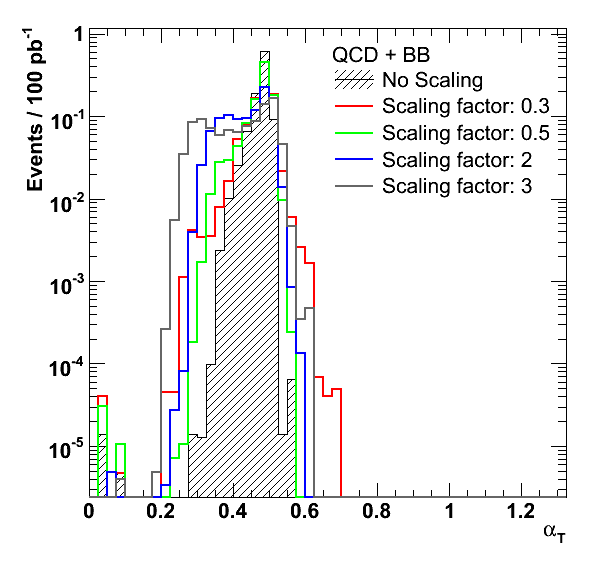
\includegraphics[scale=0.37]{./plots/aT-NT7-Scaling.png} 
\end{minipage}
%\hspace{0.5cm} % To get a little bit of space between the figures
\begin{minipage}[b]{0.5\linewidth}
\centering
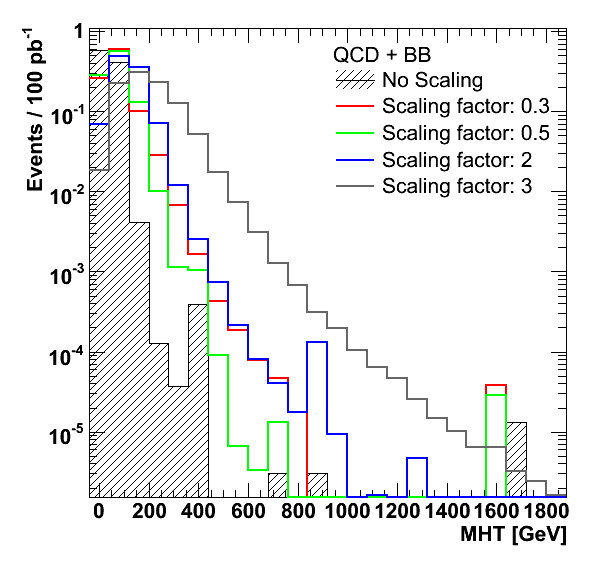
\includegraphics[scale=0.37]{./plots/MHT-NT7-Scaling.png} 
\end{minipage}
\caption{\textit{The $\alpha_{T}$ (a) and $MH_{T}$ (b) distributions after a drastic jet rescaling by different factors in QCD events. The results correspond to the extreme scenario of rescaling one jet per event.} }

\label{fig:scale1}
\end{figure}
\begin{figure}[h!]
\begin{minipage}[b]{0.5\linewidth}
\centering
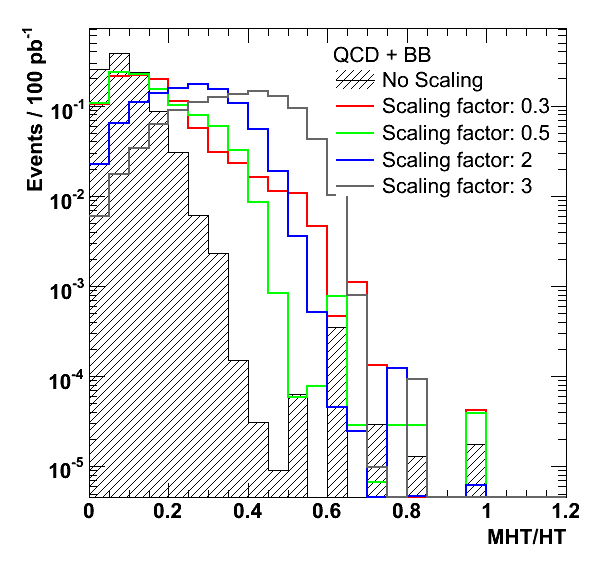
\includegraphics[scale=0.37]{./plots/MHTovHT-NT7-Scaling.png} 
\end{minipage}
%\hspace{0.5cm} % To get a little bit of space between the figures
\begin{minipage}[b]{0.5\linewidth}
\centering
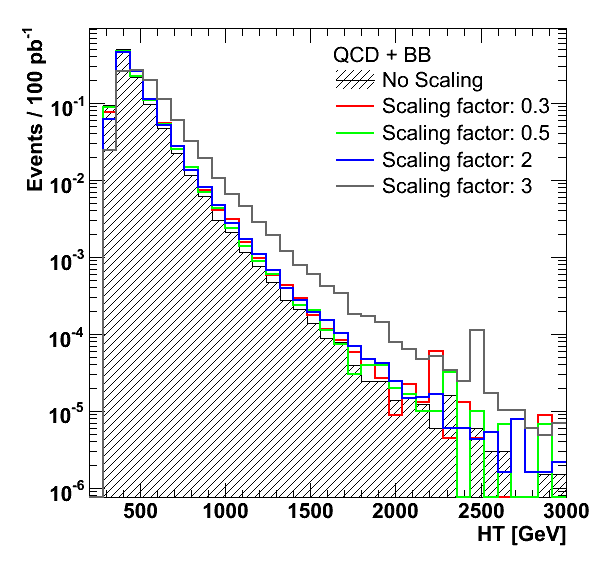
\includegraphics[scale=0.37]{./plots/HT-NT7-Scaling.png} 
\end{minipage}
\caption{\textit{The $MH_{T} / H_{T}$ (a) and $H_{T}$ (b) distributions after a drastic jet rescaling by different factors in QCD events. The results correspond to the extreme scenario of rescaling one jet per event.} }

\label{fig:scale2}
\end{figure}


In order to obtain a rough measure of the performance of the $\alpha_{T}$ versus the $MH_{T}$ approach under drastic mismeasurements of the jet energies, the following stress test was used: assuming a zero uncertainty on the measurement of the EWK background, a systematic uncertainty, $\Delta B$, assigned to the QCD component, would change the significance, $S/\sqrt{B}$, by $S/\sqrt{B + \Delta B^{2}}$. A maximum uncertainty on the QCD background ($\Delta B$) which would still allow a SUSY discovery with $\sim 5 \sigma$, can then be estimated for each final cut - an $\alpha_{T}$ or an $MH_{T}$ cut. In practise, one needs to calculate the $\Delta B$ uncertainty on QCD as a function of the probability of mis-measurement, as shown on figures ~\ref{fig:scale3} and ~\ref{fig:scale4}\footnote{If the result of $\Delta B$ is exactly 0, then the value is arbitrarily set to 0.1 because of the logarithmic scale in Y-axis.}. For each given mis-measurement fraction (scaling factor $F$) considered, the maximum rate for drastic jet mis-measurements, that would still allow a SUSY discovery, is provided in table ~\ref{tab:scale5}. Obviously, the higher the frequency by which the jet mis-measurements need to occur, the more robust the cut variable is. This favors $\alpha_{T}$ performance in almost all the cases. Rescalings by 0.1 and 0.3 factors show comparable performance between the high $MH_{T}$ cut and the $\alpha_{T}$ one, which can be understood by the indirect effect of lack of statistics (a downward scaling of the jet energies results in rejecting events due to the $H_{T}$ cut).

Therefore, the above results have demonstrated that the $\alpha_{T}$ cut performs more resilient under possibly large QCD background uncertainties.


%\newpage		

\begin{figure}[h!]
\begin{minipage}[b]{0.5\linewidth}
\centering
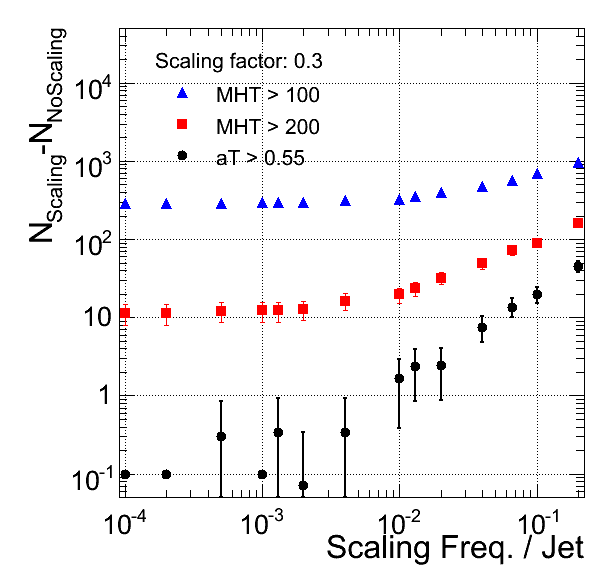
\includegraphics[scale=0.37]{./plots/DNentries_Scale03.png} 
\end{minipage}
%\hspace{0.5cm} % To get a little bit of space between the figures
\begin{minipage}[b]{0.5\linewidth}
\centering
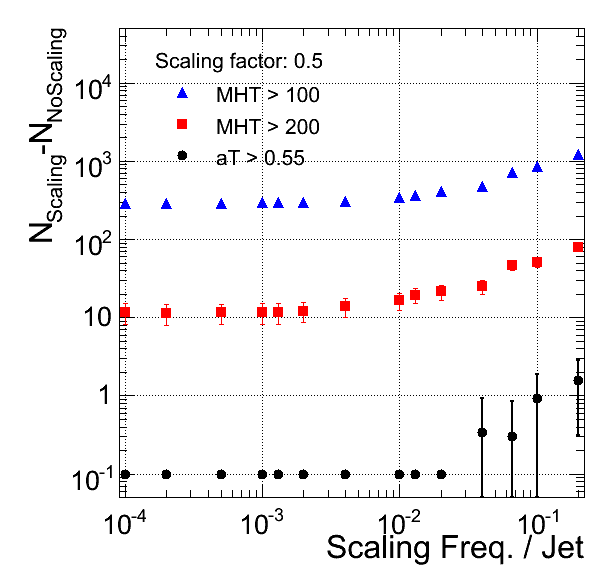
\includegraphics[scale=0.37]{./plots/DNentries_Scale05.png} 
\end{minipage}
\caption{\textit{Uncertainty on QCD background ($\Delta B$) as a function of the probability of mis-measurement, for two different down-ward scaling factors of the jet energy: 0.3 (left) and 0.5 (right).  } }
\label{fig:scale3}
\end{figure}
\begin{figure}[h!]
\begin{minipage}[b]{0.5\linewidth}
\centering
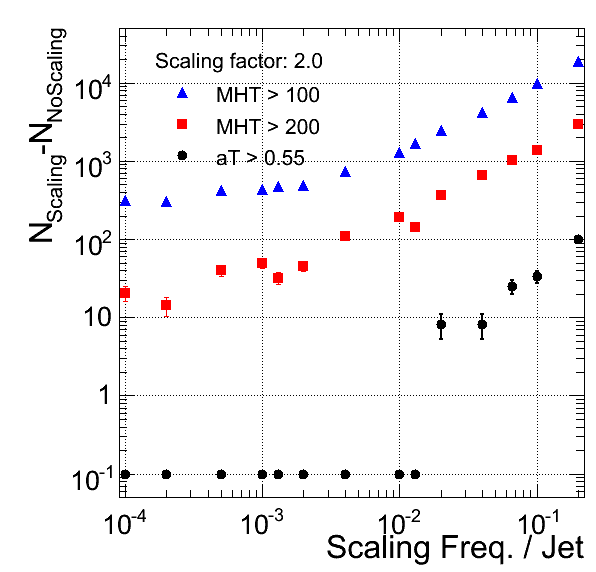
\includegraphics[scale=0.37]{./plots/DNentries_Scale2.png} 
\end{minipage}
%\hspace{0.5cm} % To get a little bit of space between the figures
\begin{minipage}[b]{0.5\linewidth}
\centering
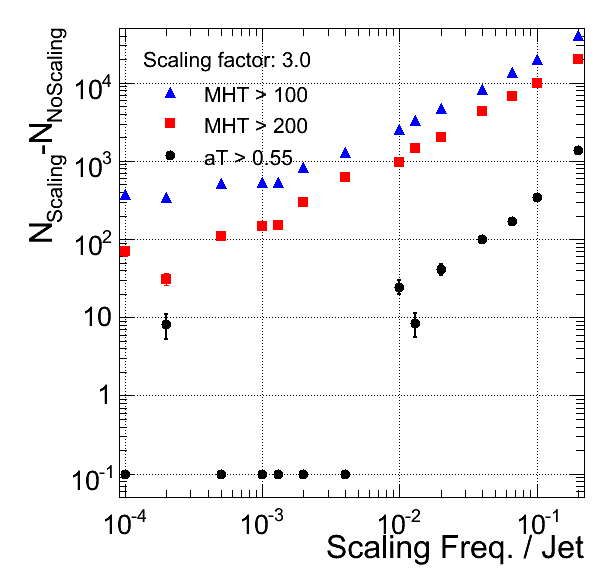
\includegraphics[scale=0.37]{./plots/DNentries_Scale3.png} 
\end{minipage}
\caption{\textit{Uncertainty on QCD background ($\Delta B$) as a function of the probability of mis-measurement, for two different up-ward scaling factors of the jet energy: 2 (left) and 3 (right).  } }
\label{fig:scale4}
\end{figure}

\begin{table}[h!]
\vspace{5mm}
\small
   \centering
   \begin{tabular}{|c||c|c|c|c|c|c|}
      \hline
 %     cut & QCD error & \multicolumn{!}{5}{Upper limit on mis-measurement rate for 5 sigma}
cut & $\Delta B$ & F=0.1 & F=0.3 & F=0.5 & F=2 & F=3 \\ \hline \hline
$MH_{T}>100$~GeV & 167.5 & $<1/10000$ & $<1/10000$ & $<1/10000$ & $<1/10000$ & $<1/10000$ \\
$MH_{T}>200$~GeV & 77. & 1/25 & 1/13 & 1/6 & 1/350 & 1/5000 \\
$\alpha_{T}>0.55$ & 11.5 & 1/50 & 1/15 & $> 1/5$ & 1/20 & 1/77 \\ \hline

   \end{tabular}
   \caption{\textit{Maximum rate of drastic jet mis-measurements, that would still allow the ``SUSY significance'' to remain $>5$, for different jet $p_{T}$ scaling factors:0.1, 0.3, 0.5, 2 and 3. }}
   \vspace{5mm}
\label{tab:scale5}
\end{table}	

Overall, despite the reduced event-yield of the $\alpha_{T}$ approach, the analysis favors in terms of robustness and reliability to control the most challenging background for LHC (QCD). In parallel, this approach avoids questions of $ME_{T}/MH_{T}$-based analyses, like where to place the cut and how to control the QCD tails and therefore can be considered as a reliable alternative method to the traditional RA4-like approaches.



%\newpage
\begin{comment}

\begin{table}[h!]
   \centering
   \begin{tabular}{|c||c|c|c|c|c|c|c|}
      \hline
& QCD & $b\bar{b}+\textrm{jets}$ & $Z+\textrm{jets}$ & $W+\textrm{jets}$ & $t\bar{t} + \textrm{jets}$ & LM1 & LM0 \\ \hline
no smearing & 0 & 1.4 & 0.6 & 23.8 & 13. & 40.1 & 66.7 \\ \hline
scaling factor 0.3 & 67.6 & 11.7 &0 &16.8 &15.7 &26.8 &51.4 \\ \hline
scaling factor 0.5 & 1.9 & 0.5 & 0 & 11.5 & 10.4 &30.9 & 46.4 \\ \hline
scaling factor 2 & 49.8 & 13. & 2.3 & 82.9 & 59. & 43.2 &95.7 \\ \hline
scaling factor 3 & 379.3 & 90.7 & 7.9 & 174.4 & 124.1 & 41.1 & 118.5 \\ \hline
   \end{tabular}
   \caption{\textit{Expected number of events after the pre-selection cuts and an $\alpha_{T}>0.55$ cut, for all the background processes (QCD, $b\bar{b}$+jets, W/Z + jets, $t\bar{t}$+jets) and the SUSY LM1 and LM0. The final numbers correspond to the default case (no jet smearing) and the cases of the $p_{T}$ scaling of 1 randomly selected jet by a constant factor of 0.3, 0.5, 2 and 3. }}
\end{table}			

\begin{table}[h!]
   \centering
   \begin{tabular}{|c||c|c|c|c|c|c|c|}
      \hline
& QCD & $b\bar{b}+\textrm{jets}$ & $Z+\textrm{jets}$ & $W+\textrm{jets}$ & $t\bar{t} + \textrm{jets}$ & LM1 & LM0 \\ \hline
no smearing & 12.2 & 2.3  & 0.3 & 53.8 & 33.3 & 107.8 & 217.2 \\ \hline
scaling factor 0.3 & 274.2 & 28.7 & 2. & 48.8 &40. &75.6 & 173.2 \\ \hline
scaling factor 0.5 & 121.6 & 12.4 & 1.7 & 47.6 & 32.1 &86.7 & 168.7 \\ \hline
scaling factor 2 & 4878.1 & 833.9 & 26.7 & 509.8 & 242.4 & 137.1 & 396.8 \\ \hline
scaling factor 3 & 33170. & 5828.2 & 105.2 &1420.9 & 728. & 151. &551.1 \\ \hline
   \end{tabular}
   \caption{\textit{Expected number of events after the pre-selection cuts and an $MH_{T}>200$ GeV cut, for all the background processes (QCD, $b\bar{b}$+jets, W/Z + jets, $t\bar{t}$+jets) and the SUSY LM1 and LM0. The final numbers correspond to the default case (no jet smearing) and the cases of the $p_{T}$ scaling of 1 randomly selected jet by a constant factor of 0.3, 0.5, 2 and 3.}}
\end{table}			

\end{comment}

